%-------------------------
%minimal-unix
%(c) H.Buchmann FHNW 2014
%export TEXINPUTS=${HOME}/fhnw/edu/:${HOME}/fhnw/edu/tinL/config/latex:${HOME}/fhnw/edu/config//:
%-------------------------
\documentclass{beamer}
\usepackage{latex/beamer}
%---------------------
%local defines
%(c) H.Buchmann FHNW 2009
%$Id$
%---------------------
\newcommand{\target} {\beaglebone\xspace}
\newcommand{\targetS}{{\bf BBG}\xspace}
\newcommand{\host}   {{\em Host}\xspace}
\newcommand{\targetroot} {{\bf target-root}\xspace}
\newcommand{\kernel} {{\bf kernel}\xspace}
\renewcommand{\c}{{\bf C}\xspace}
\newcommand{\cpp}{{\bf C++}\xspace}
\newcommand{\posix}{{\bf POSIX}\xspace}

\input{/home/buchmann/latex/dirtree/dirtree.tex}

\usepackage[absolute]{textpos}
\setlength{\TPHorizModule}{1mm}
\setlength{\TPVertModule}{1mm}

\begin{document}

\newcommand{\qemu}{{\em qemu}\xspace}
\newcommand{\busybox}{{\em busybox}\xspace}
\newcommand{\yocto}{{\em yocto}\xspace}
\title{Zugriff auf die Hardware}

\frame{\titlepage}

\begin{frame}{Um was geht es ?}{Zugriff auf mehrere Arten}
 \begin{itemize}
  \item userspace
  \begin{itemize}
   \item per \cod{/sys/class/gpio}
   \item per \cod{mmap} mit eigenem Programm: 
  \end{itemize}
  \item kernelspace
  \begin{itemize}
   \item mit eigenem module
  \end{itemize}
 \end{itemize}
\end{frame}

\section{Userspace}
\subsection{sys/class/gpio}
\begin{frame}{\cod{sys/class/gpio}}
 \begin{itemize}
  \item \cod{kernel/Documentation/gpio.txt}
  \item Gute Pins:
   \begin{itemize}
    \item 35: PWR\_LED
    \item 47: ACT\_LED
   \end{itemize}
 \end{itemize}
\end{frame}

\subsection{mmap}
\begin{frame}{\cod{mmap}}{Direkter Zugriff auf die Hardware}
 \begin{itemize}
  \item Beschreibung
   \begin{itemize}
    \item BCM2835 ARM Peripherals (BCM2835-ARM-Peripherals.pdf) Abschnitt 6
   \end{itemize}
  \item Wo im Speicher
   \begin{itemize}
    \item \cod{/proc/iomem}
   \end{itemize}
 \item Der wichtige Aufruf
  \begin{itemize}
   \item \cod{mmap}
  \end{itemize}
 \end{itemize}
\end{frame}

\begin{frame}[fragile]{mmap}
\begin{center}
 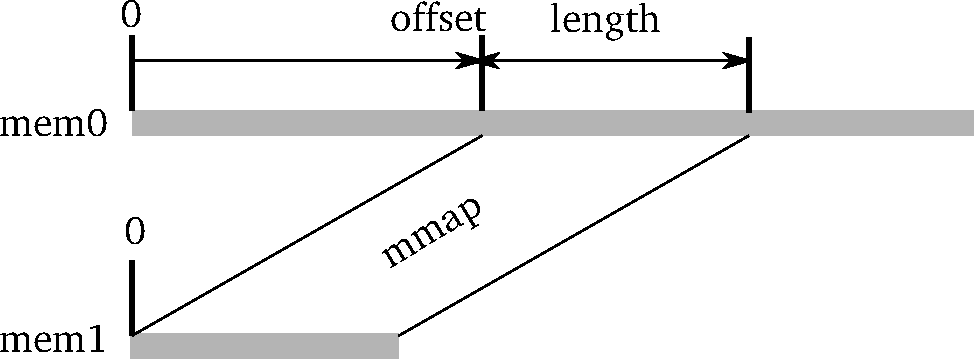
\includegraphics[width=8cm]{mmap.pdf}
\end{center}
\begin{lstlisting}[language=C]
 mem=(unsigned char*)mmap(0, /* addr hint */
     length,
     PROT_READ|PROT_WRITE,
     MAP_SHARED, 
     memId,
     offset);
\end{lstlisting}
\end{frame}

\begin{frame}{Aufgabe}
 \begin{itemize}
  \item \cod{gpio.sh}:  \cod{sys/class/gpio}
  \item \cod{blink.sh}: \cod{mmap}
 \end{itemize}
\end{frame}

\end{document}
